\begin{quote}
Aenean ullamcorper risus id libero. Pellentesque ac sem eget libero aliquam tincidunt. Suspendisse neque. Rutrum id, faucibus vitae, leo. Donec ut wisi. Vivamus ornare, lorem quis tristique dapibus, nulla nisl nonummy libero, vitae luctus sem felis vel nisl. Suspendisse lectus lacus, ultricies vitae, feugiat et, hendrerit in, quam. Pellentesque porttitor enim at lectus. Praesent viverra laoreet velit. Mauris neque odio, ornare id, rhoncus non, sollicitudin sed, lectus. Aenean ullamcorper risus id libero. Pellentesque ac sem eget libero aliquam tincidunt. Suspendisse neque\footcite[voir \pno~154]{Georges1974}.
\end{quote}

blabla massa\footcite[12]{Pierre1901}

\begin{figure}[htbp]
   \begin{center}
      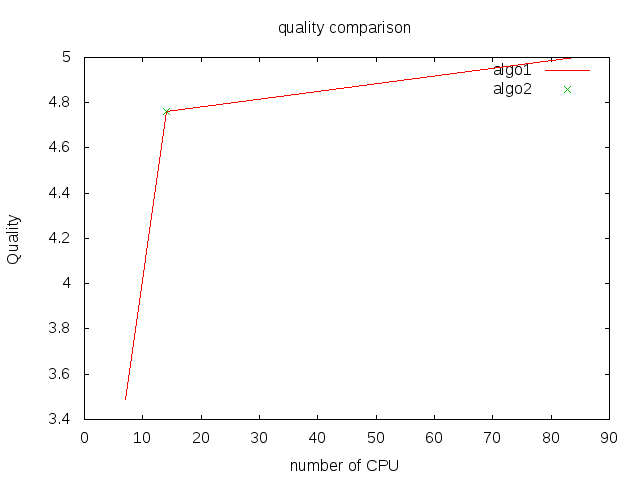
\includegraphics[width=0.8\linewidth]{Chapitre1/figures/comparison.png}
   \end{center}
   \caption[titre court pour la liste des figures]
   {\footnotesize Titre plus long avec des explications.}
   \label{fig:mafigure2}
\end{figure}

\begin{verse}
Maître Corbeau, sur un arbre perché, \\
Tenait en son bec un fromage. \\
Maître Renard, par l'odeur alléché, \\
Lui tint à peu près ce langage : \\
«~Hé ! bonjour, Monsieur du Corbeau. \\
Que vous êtes joli ! que vous me semblez beau ! \\
Sans mentir, si votre ramage \\
Se rapporte à votre plumage, \\
Vous êtes le Phénix des hôtes de ces bois.~» \\
\end{verse}

\boitemagique{Titre de la boite}{
Praesent placerat, ante at venenatis pretium, diam turpis faucibus arcu, nec vehicula quam lorem ut leo. Sed facilisis, augue in pharetra dapibus, ligula justo accumsan massa, eu suscipit felis ipsum eget enim.
}

\boitesimple{Mauris lorem quam, tristique sollicitudin egestas sed, sodales vel leo. In hac habitasse platea dictumst. Lorem ipsum dolor sit amet, consectetur adipiscing elit. Sed sed lorem lacus, at venenatis elit. Pellentesque nisl arcu, blandit ac eleifend non, sodales a quam.}

